%%%%%%%%%%%%%%%%%%%%%%%%%%%%%%%%%%%%%%%%%
% My Moleskine Basic Template
% LaTeX Template
% 
% for Moleskine page size: large 13x21 cm 
% Version 0.1
%
% This template is available at:
% http://www.github.com/hannic
%
% License:
% CC BY-NC-SA 3.0 (http://creativecommons.org/licenses/by-nc-sa/3.0/)
%
% Compiling this template:
% When you first open the template, compile it from the command line with the 
% commands below to make sure your LaTeX distribution is configured correctly:
%
% 1) lorem ipsum
% 2) lorem ipsum
%
% This template also uses a number of packages which may need to be
% updated to the newest versions for the template to compile. It is strongly
% recommended you update your LaTeX distribution if you have any
% compilation errors.
% 
% * Layout size (page size) defined by using package geometry and \geometry command 
% * Define color "my-grey" for Text 
%
%%%%%%%%%%%%%%%%%%%%%%%%%%%%%%%%%%%%%%%%%

%----------------------------------------------------------------------------------------
% !!!! = my helper shortcuts etc = !!!!
% 
% cmd + alt => vertical selection 
%----------------------------------------------------------------------------------------


%----------------------------------------------------------------------------------------
% PACKAGES AND OTHER DOCUMENT CONFIGURATIONS
%----------------------------------------------------------------------------------------
\documentclass[english,a4paper]{article}
\usepackage{geometry}
\usepackage{fontawesome}

\geometry{a4paper, layoutwidth=17cm, layoutheight=28cm}
\usepackage{fancybox}
\usepackage{babel}
\usepackage{lastpage}
\usepackage{fancyhdr}
\usepackage{afterpage}
\usepackage{fancyhdr}
\usepackage{xcolor}                     % https://en.wikibooks.org/wiki/LaTeX/Colors
\usepackage[utf8]{inputenc}
\usepackage[T1]{fontenc}
\definecolor{my-grey}{HTML}{696969}     
\usepackage[absolute]{textpos}
\usepackage[skins]{tcolorbox}
\usepackage{lipsum}
\usepackage{%
    ngerman,
    graphicx,
    url,
    lmodern,
    fontenc,
    paralist,
    pifont,
    amsmath,amssymb,latexsym,           % http://zelmanov.ptep-online.com/ctan/symbols.pdf
                                        % https://sites.math.washington.edu/~reu/docs/latex_symbols.pdf
    marvosym, dashrule,                  % dashrule for dotted underlines 
                                        % http://tug.ctan.org/macros/latex/contrib/dashrule/dashrule.pdf
    pifont
    }
\DeclareFontFamily{U}{hands}{}    % http://tug.ctan.org/info/symbols/comprehensive/symbols-a4.pdf
\DeclareFontShape{U}{hands}{m}{n}{<-> hands}{} 
\DeclareFontFamily{U}{dancers}{}    
\DeclareFontShape{U}{dancers}{m}{n}{<-> dancers}{}

% === path to graphics
\graphicspath{ {images/} }

% === smartdiagram
\usepackage{smartdiagram}

% === shapes
\usepackage{tikz}
\usetikzlibrary{shapes}
\usetikzlibrary[positioning]
\usetikzlibrary{patterns}
\usepackage{verbatim}

%----------------------------------------------------------------------------------------
% DEFINE PAGESTYLE
%----------------------------------------------------------------------------------------
\pagestyle{fancy}

\color{my-grey}

% clear any old style settings
\fancyhead{}
\fancyfoot{}

% define new headers/footers
\lhead{\tiny Moleskine Template (Size: Large) }
\rhead{\tiny \today}
\lfoot{\huge \hspace{0.25cm} \Rightscissors \hspace{0.55cm}}
\rfoot{\tiny \thepage\ of \pageref{LastPage}}


% define layout 
% thin border with rounded corner  (fancybox > ovalbox)
\fancypage{ \setlength{\fboxsep}{5pt}\ovalbox}{}

% === item overwritten used with "itemize"
\renewcommand{\labelitemi}{$\bigcirc$}
\renewcommand{\labelitemii}{\ding{74}}

\newcommand{\daywidth}{0.6 cm}


%----------------------------------------------------------------------------------------
% BEGIN DOCUMENT
%----------------------------------------------------------------------------------------
\begin{document}
\thispagestyle{fancy}
%----------------------------------------------------------------------------------------
% CONTENTS
%----------------------------------------------------------------------------------------

\begin{center}

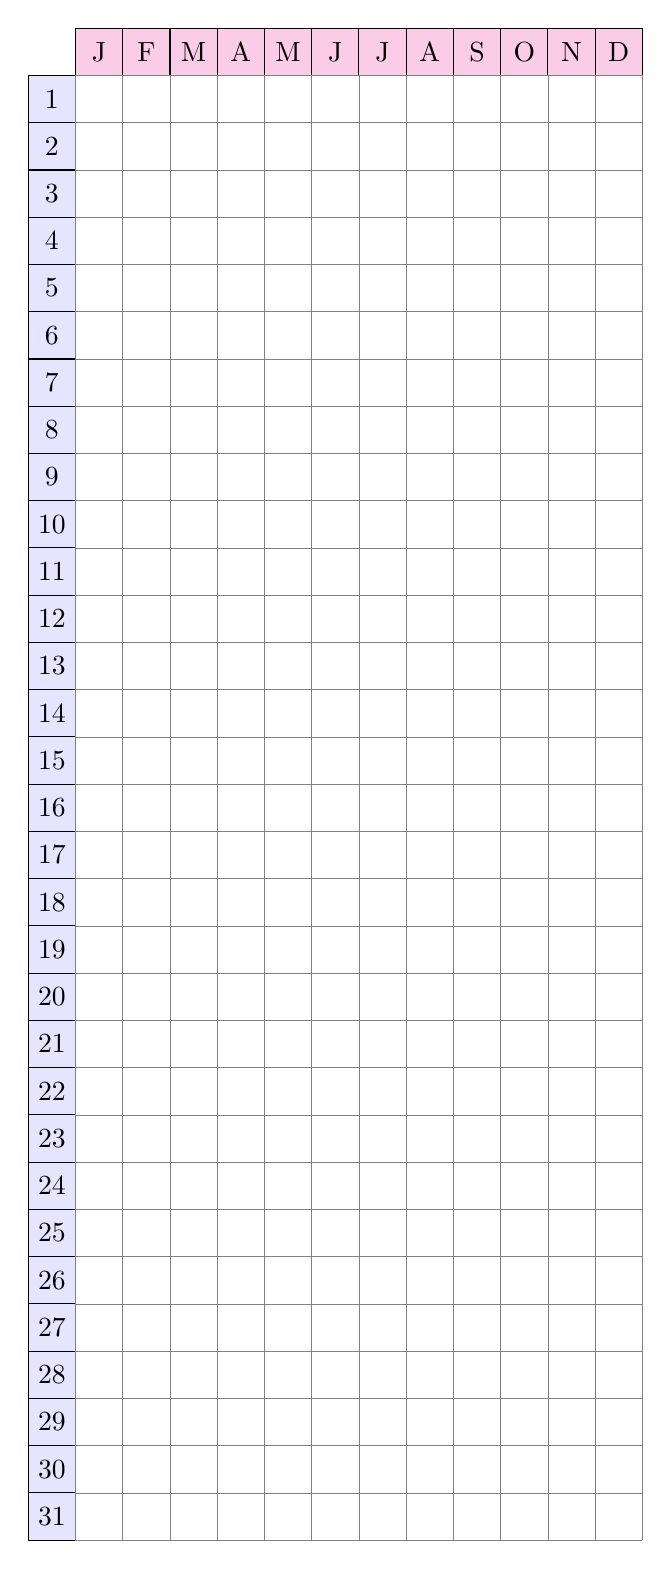
\begin{tikzpicture}[x=\daywidth, y=-0.6cm, node distance=0 cm,outer sep = 0pt]
% Style for Days
\tikzstyle{day}=[draw, rectangle,  minimum height=0.6cm, minimum width=\daywidth, fill=magenta!20,anchor=south west]
% Style for hours
\tikzstyle{hour}=[draw, rectangle, minimum height=0.6 cm, minimum width=0.6 cm, fill=blue!10!white,anchor=north east]

% Styles for events
% Duration of sequences
\tikzstyle{hours}=[rectangle,draw, minimum width=\daywidth, anchor=north west,text centered,text width=1 em]
\tikzstyle{1hour}=[hours,minimum height=0.6cm]
\tikzstyle{2hours}=[hours,minimum height=1.4cm]
\tikzstyle{3hours}=[hours,minimum height=2.1cm]
%Style for type of sequence 
\tikzstyle{Ang2h}=[1hour,fill=green!20]
\tikzstyle{Phys2h}=[2hours,fill=red!20]
\tikzstyle{Math2h}=[2hours,fill=blue!20]
\tikzstyle{TIPE2h}=[2hours,fill=blue!10]
\tikzstyle{TP2h}=[2hours, pattern=north east lines, pattern color=magenta]
\tikzstyle{G3h}=[3hours, pattern=north west lines, pattern color=magenta!60!white]
\tikzstyle{Planche}=[1hour,fill=white]
\tikzstyle{Lunch}=[1hour,fill=white]
\tikzstyle{Freetime}=[1hour,fill=magenta!80!white]
\tikzstyle{Evening}=[2hours, pattern=north west lines, pattern color=magenta]


% Positioning labels for days and hours
\node[day] (Jan) at (1,8) {J};
\node[day] (Feb) [right = of Jan] {F};
\node[day] (Mar) [right = of Feb] {M};
\node[day] (Apr) [right = of Mar] {A};
\node[day] (Mai) [right = of Apr] {M};
\node[day] (Jun) [right = of Mai] {J};
\node[day] (Jul) [right = of Jun] {J};
\node[day] (Aug) [right = of Jul] {A};
\node[day] (Sep) [right = of Aug] {S};
\node[day] (Oct) [right = of Sep] {O};
\node[day] (Nov) [right = of Oct] {N};
\node[day] (Dec) [right = of Nov] {D};


\node[hour] (8-9) at (1,8) {1};
\node[hour] (9-10) [below = of 8-9] {2};
\node[hour] (10-11) [below= of 9-10] {3};
\node[hour] (11-12) [below = of 10-11] {4};
\node[hour] (12-13) [below  = of 11-12] {5};
\node[hour] (13-14) [below = of 12-13] {6};
\node[hour] (14-15) [below = of 13-14] {7};
\node[hour] (15-16) [below = of 14-15] {8};
\node[hour] (16-17) [below = of 15-16] {9};
\node[hour] (17-18) [below = of 16-17] {10};
\node[hour] (18-19) [below = of 17-18] {11};

\node[hour] (20-11) [below= of 18-19] {12};
\node[hour] (21-12) [below = of 20-11] {13};
\node[hour] (22-13) [below  = of 21-12] {14};
\node[hour] (23-14) [below = of 22-13] {15};
\node[hour] (24-15) [below = of 23-14] {16};
\node[hour] (25-16) [below = of 24-15] {17};
\node[hour] (26-17) [below = of 25-16] {18};
\node[hour] (27-18) [below = of 26-17] {19};
\node[hour] (28-19) [below = of 27-18] {20};

\node[hour] (30-11) [below= of 28-19] {21};
\node[hour] (31-12) [below = of 30-11] {22};
\node[hour] (32-13) [below  = of 31-12] {23};
\node[hour] (33-14) [below = of 32-13] {24};
\node[hour] (34-15) [below = of 33-14] {25};
\node[hour] (35-16) [below = of 34-15] {26};
\node[hour] (36-17) [below = of 35-16] {27};
\node[hour] (37-18) [below = of 36-17] {28};
\node[hour] (38-19) [below = of 37-18] {29};
\node[hour] (48-19) [below = of 38-19] {30};
\node[hour] (58-19) [below = of 48-19] {31};

%Position of sequences
%\node[Lunch] at (1,8) { }; % {Anglais}
\draw[step=0.6cm,style=help lines] (1,8) grid (13,39);

% \node[Phys2h] at (1,8) { };
% \node[Phys2h] at (2,8) { };
% \node[Phys2h] at (4,8) { };
% \node[Phys2h] at (5,10) { };
% \node[Math2h] at (2,10) { };
% \node[Math2h] at (2,14) { };
% \node[Math2h] at (3,8) { };
% \node[Math2h] at (4,10) { };
% \node[Math2h] at (5,8) { };
% \node[TIPE2h] at (1,14) { };
% \node[TIPE2h] at (1,16) { };
% \node[TIPE2h] at (2,16) { };
% \node[TIPE2h] at (3,10) { };
% \node[TIPE2h] at (5,14) { };
% \node[TIPE2h] at (5,16) { };
% \node[TP2h] at (3,14) { };
% \node[TP2h] at (3,16) { };
% \node[Lunch] at (1,12) { Lunch time };
% \node[Lunch] at (2,12) { Lunch time };
% \node[Lunch] at (3,12) { Lunch time };
% \node[Lunch] at (4,12) { Lunch time };
% \node[Lunch] at (5,12) { Lunch time };
% 
% %\node[Lunch] at (4,12) { Lunch time };
% 
% \node[Freetime] at (1,18) { Freetime };
% \node[Freetime] at (3,18) { Freetime };
% \node[Freetime] at (5,18) { Freetime };
% 
% \node[Evening] at (2,18) { };
%\node[Planche] at (4,13.5) { Lunch time};
\end{tikzpicture}   
\end{center}


%\Pisymbol{hands}{65}
%\Pisymbol{dancers}{40}

\end{document}

